\pdfoutput=1 % only if pdf/png/jpg images are used
\documentclass{JINST}

\usepackage{amsmath,amssymb}
\usepackage[numbers,sort]{natbib}
%\hypersetup{colorlinks, citecolor=blue, linkcolor=blue, filecolor=blue, urlcolor=red}

\title{Improved Background Rejection in Neutrinoless Double Beta Decay Experiments with Gaseous Xenon Detectors}

\author{A. Author$^a$,
B. Author$^a$\thanks{Corresponding author.}~
and C. Author$^b$\\
\llap{$^a$}Instituto de F\'isica Corpuscular (IFIC), CSIC \& Universitat de Val\`encia,\\ 
Calle Catedr\'atico Jos\'e Beltr\'an, 2, 46980 Paterna, Valencia, Spain\\
\llap{$^b$}Name of Institute,\\
  Address, Country\\
E-mail: \email{CorrespondingAuthor@email.com}}

\bibliographystyle{unsrtnat}

\abstract{We propose a potential improvement in background rejection capability of neutrinoless double-beta ($0\nu\beta\beta$) decay experiments conducted with high-pressure xenon gas detectors capable of imaging electron tracks.  The improvement relies on the ability to distinguish the different track signatures left by single-electron (background) events and two-electron ($0\nu\beta\beta$) events in such a detector in the presence of an external magnetic field.  This initial study shows that, by analyzing the curvature of the reconstructed helical tracks, a potentially significant additional background rejection factor can be obtained with an acceptable loss in signal efficiency.}

\keywords{Neutrinoless double beta decay; Kalman filter; particle tracking}

\begin{document}

\section{Introduction}\label{sec:intro}
% Significant push on 0vbb (EXO, KLZ, GERDA) and others (CUORE, NEXT) incoming (look at recent paper, talk to Justo); talking about 100 kg or at most few hundred per year.  Typically total # bg. counts / ton / yr of order a few to few tens of counts (in paper and Justo's thesis); GERDA is 0.01 cts/keV/kg/yr, NEXT has 10^-4 cts/kg/year 10 keV*10^-4 gives 5 cts, factor of 5 or more and we'd be in the range of 1 count.  Can we still improve HPXe technologoy?  What are our current limitations (diffusion, think we can get 0.5 %, difficult to hit the Fano factor, close to intrinsic); can topological signal be improved (diffusion is problem), makes any analysis difficult (7mm); diffusion can be reduced to 1-3mm without losing energy resolution by additives... is it possible to imrprove further (this would already improve the blob): will Bfield give us an extra handle: explore this capability with 1-3 mm resolution, scanning B, P
% Want to demonstrate 1-2 cts/ton/year; 12 keV * 10^-4 ... we currently have 5e-4, want to get 1e-4; new factor of 5
% Want to finish paper by next week + talk 
% Next: profile approach rather than asymmetry factor; and finding vertex
Double beta decay refers to one of two processes in which two simultaneous $\beta$-decays occur within a nucleus and
may be an accessible mode of decay in candidate isotopes for which the single-beta decay mode is forbidden or highly
suppressed due to the energetics of the relevant nuclear configurations.  In one such process referred to as two-neutrino
double-beta decay, two electrons are emitted along with two antineutrinos,

\begin{equation}
 (Z,A) \rightarrow (Z+2,A) + 2e^{-} + 2\bar{\nu}_{e}.
\end{equation}

This process is allowed in the Standard Model and has been observed in several nuclei.  Double-beta decay has also been
postulated to exist in the zero-neutrino mode, or neutrinoless double-beta ($0\nu\beta\beta$) decay, in which the two 
antineutrinos are not emitted as a product of the reaction and the total energy released in the decay, $Q_{\beta\beta}$, is 
given to the two electrons.  The observation of $0\nu\beta\beta$ would have several significant implications
in fundamental physics.  The decay cannot occur unless the neutrino is a Majorana particle, that is, unless it is
physically equivalent to its anti-particle.  Majorana neutrinos would be evidence for new physics at an energy scale
inversely proportional to the neutrino masses, and their existence violates the conservation of total lepton number. 
Furthermore, lepton number violation combined with CP violation could explain the excess of matter over anti-matter
present in the universe via the mechanism known as leptogenesis.  $0\nu\beta\beta$ decay has been frequently revisited
in reviews (see for example \cite{Cadenas_2012, Bilenky_2010, Elliot_2012}).

Many experimental challenges accompany these far-reaching physics implications.  No confirmed observation of
$0\nu\beta\beta$ has yet been made, though it has received much recent experimental attention.   The current 
generation of experiments operate with tens to several hundred kilograms of candidate isotope mass.  Some of these
experiments such as EXO \cite{EXO_2012, EXOPRL_2012}, GERDA \cite{GERDA_2004, GERDA_2013}, and KamLAND-Zen 
\cite{KamLANDZen_2012, KamLANDZen_2013} are already running and have directly observed the $2\nu\beta\beta$ 
mode in their chosen candidate isotope and set new lower limits on the half-life for $0\nu\beta\beta$ decay.  Others are 
still in the prototype or construction phases including CUORE \cite{CUORE_2015}, MAJORANA \cite{MAJORANA_2013}, 
NEXT \cite{NEXT_2014}, SNO$+$ \cite{SNOPLUS_2014}, and SuperNEMO \cite{SuperNEMO_2010}.  Because no signal
has yet been seen in experiments employing hundreds of kilograms of candidate isotope, it may be necessary to 
design a low-background experiment capable of operating with tonnes of candidate isotope to continue searching
for the decay.  The different technological strategies used in the current wide variety of $0\nu\beta\beta$
experiments may not be applicable at the tonne-scale, and such technologies would need to demostrate a clear
ability to scale upward in size before being considered for a tonne-scale experiment.

%The $0\nu\beta\beta$ experiment NEXT will use 100 kg of xenon enriched in the candidate isotope $^{136}$Xe in a
%high pressure xenon time projection chamber (TPC).  A tracking plane consisting of silicon photomultipliers (SiPMs)
%will be used to reconstruct ionization tracks in $(x,y)$, while the $z$-coordinate is determined using the drift time of
%electrons in a readout scheme based on electroluminescence (EL).  A resolution in $(x,y,z)$ of several mm is anticipated,
%and therefore the techniques developed here should be directly applicable to such an experiment.

\section{Motivation}
\subsection{Background Rejection in Double-Beta Experiments}
In recent $0\nu\beta\beta$ experiments, the total number of background events observed or expected in the energy 
region of interest has been on the order of a few counts to a few tens of counts per year.  The NEXT experiment will use a 
high pressure xenon time projection chamber (TPC) to search for $0\nu\beta\beta$ decay
using 100 kg of xenon enriched in the candidate isotope $^{136}$Xe.  The experiment currently 
expects a background rate of $5 \times 10^{-4}$ counts/keV/kg/year, and for a 10 keV region of interest and 100 kg of 
isotope, 5 counts/year.  To improve sensitivity at the current scale and in anticipation of a larger mass detector, we ask
if this rate could possibly be reduced further.  One potential improvement would be in energy resolution, narrowing the
energy region of interest and therefore the total background rate.  Xenon has been shown to have very good intrinsic 
energy resolution in the gas phase \cite{Bolotnikov}, and the current energy resolution achieved in NEXT prototypes 
using the low-noise electroluminescent (EL) gain process has not yet reached the intrinsic level \cite{NEXT_2013}.  
Improvements particularly in photon collection and detection statistics could further improve the energy resolution and 
therefore the observed background rate in high pressure xenon TPCs.  

The present study will focus on a different approach to background rejection in which the one-electron background 
events and two-electron double beta events are distinguished by examining the signature of the track left by the event in 
the detector.  The energetic electrons produced in $0\nu\beta\beta$ decay deposit their energy as they travel through 
the xenon gas, leaving a track of ionization in their path.  Because the ionization density $dE/dx$ is greater at lower 
electron energies, the two ends of the electron tracks are marked by two ``blobs'' of greater ionization density.  For a 
single-electron track, only one ionization track with one ``blob'' is produced.  This difference in track signatures can be 
used to distinguish between background events, for example due to high-energy gamma rays, that produce 
single-electron tracks, and double-beta events.\footnote{Note that this track signature is present for both 
$0\nu\beta\beta$ and $2\nu\beta\beta$ events, and so it cannot be used to reject background events from the 
two-neutrino mode.  For this one must rely on good energy resolution.}  Such studies based on identification of the two 
``blobs'' have already shown that the track signatures can be used to reject background events.  In this study we 
compare the single and double-electron track signatures in the presence of an applied external field and quantify the 
additional ability to reject single-electron events that is gained by examining the curvature of the tracks induced by the 
field.

We note that the ability to conduct a detailed study of the reconstructed track is highly dependent on the resolution
with which the track can be reconstructed in the detector.  One major limiting factor in tracking resolution is the diffusion
of electrons in the gas.  The ionization track produced in some active volume must be drifted to a readout plane and 
therefore the electrons may diffuse significantly and limit the resolution with which the track can ultimately be
reconstructed.  The use of an additive quenching gas may serve to reduce the diffusion to a level that would allow
good resolution of the helical motion of an electron track in a magnetic field.

%Typically total # bg. counts / ton / yr of order a few to few tens of counts (in paper and Justo's thesis); GERDA is 0.01 cts/keV/kg/yr, NEXT has 10^-4 cts/kg/year 10 keV*10^-4 gives 5 cts, factor of 5 or more and we'd be in the range of 1 count.  Can we still improve HPXe technologoy?  What are our current limitations (diffusion, think we can get 0.5 %, difficult to hit the Fano factor, close to intrinsic); can topological signal be improved (diffusion is problem), makes any analysis difficult (7mm); diffusion can be reduced to 1-3mm without losing energy resolution by additives... is it possible to imrprove further (this would already improve the blob): will Bfield give us an extra handle: explore this capability with 1-3 mm resolution, scanning B, P
 % Want to demonstrate 1-2 cts/ton/year; 12 keV * 10^-4 ... we currently have 5e-4, want to get 1e-4; new factor of 5

\subsection{Particle Tracks in Xenon in a Magnetic Field}\label{ssec:magmotion}
% Note that we could measure curvature in absence of MS; but even with MS the sign can be determined
A particle of charge $q$ moving at a velocity $\mathbf{v}$ in the presence of a magnetic field $\mathbf{B}$ is acted 
upon by a force

\begin{equation}
\mathbf{F} = q(\mathbf{v} \times \mathbf{B}).
\end{equation}

This force will cause an electron to execute helical motion in the magnetic field such that if the thumb of the right hand is positioned along the direction of the field line $\mathbf{B}$ the electron will spiral in the direction in which the fingers curl when closed around the field line (see figure \ref{fig_bfieldmotion}).  The frequency of rotation about the field line is known as the cyclotron frequency $\omega_{\mathrm{cyc}} = qB/m$, where $B$ is the magnitude of the applied magnetic field $B = |\mathbf{B}|$ and $m$ is the mass of the charged particle.
% radius of curvature $r = p_{T}/qB$

\begin{figure}[!htb]
	\centering
	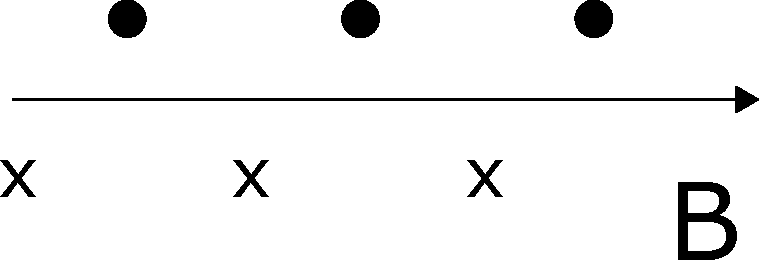
\includegraphics[scale=0.48]{fig/bfield_motion.pdf}
	\caption{\label{fig_bfieldmotion}Motion of an electron in a magnetic field.  The electron exhibits helical motion around the field line as shown (entering the page at the $\times$ and exiting the page at the $\bullet$) regardless of the direction of the component of the electron's velocity along the direction of $\mathbf{B}$.}
\end{figure}

In the presence of an applied external magnetic field, the ionization track produced by an energetic electron moving 
through high pressure xenon gas will be a helix with some alterations due to electron multiple scattering.  If the direction
of the applied magnetic field is known, the curvature of the track can be calculated to determine whether the component
of the electron velocity along the magnetic field is parallel or antiparallel to the field.  The curvature $\kappa$ can 
be calculated for track coordinates $(x,y,z)$ as

\begin{equation}\label{eqn_curv}
\kappa = \frac{(dx/dz)\cdot(d^2y/dz^2) - (dy/dz)\cdot(d^2x/dz^2)}{\Bigl[(dx/dz)^2 + (dy/dz)^2\Bigr]^{3/2}}.
\end{equation}

With this definition, an electron traveling in the direction of the magnetic field will spiral around the field lines with positive curvature, while an electron traveling opposite the direction of the magnetic field will spiral with negative curvature.  The curvature, however, will be of the opposite sign if the track orientation is not properly identified in the calculation (i.e., if $dz$ is of the wrong sign).  Thus, when calculating the curvature of a single-electron track, one would expect $\kappa > 0$ for $dz > 0$ and $\kappa < 0$ for $dz < 0$ given that $dz$ is always in the direction of the electron velocity.  However, for a $0\nu\beta\beta$ track, taking one of the extremes to be the beginning of the track and the other to be the end will lead to a calculation of $\kappa$ assuming the wrong track orientation for one of the two electrons, as the vertex at which the reaction occured is found somewhere on the interior of the track.  Therefore one expects to find $\kappa < 0$ for $dz < 0$ and $\kappa > 0$ for $dz > 0$ for a significant fraction of the track.  This difference in the behavior of the calculated curvature of reconstructed tracks will allow for the separation of single-electron and $0\nu\beta\beta$ events.

One serious limitation to this strategy is the presence of electron multiple scattering.  This is the process by which
an energetic electron is scattered repeatedly while traveling through the xenon gas and can result in deviations of its
path by significant angles.  The process can be modeled by, assuming the electron is traveling along an axis in the $\hat{\mathbf{z}}$ direction, considering the angle of deflection projected on the $x$ and $y$ planes when scattered
through a thickness of xenon $x$.  Each of these angles $\theta_x$ and $\theta_y$ can be modeled by a gaussian 
distribution as

\begin{equation}\label{eqn_mscat}
\sigma^{2}(\theta_{x,y}) = \frac{13.6\,\,\mathrm{MeV}}{\beta p}\sqrt{dz/L_{0}}\bigl[1 + 0.038\ln(dz/L_{0})\bigr],
\end{equation}

\noindent for an electron with momentum $p$ in MeV/c before scattering and beta factor $\beta$ (where $c = 1$).
$L_{0}$ is the radiation length, a property of the medium.  Without the influence of multiple scattering, the track of
an energetic electron would follow a helical path with a well-defined curvature, apart from noise due to diffusion and
the track reconstruction procedure.  In this case the transverse momentum could be directly determined by the
curvature as $p_{T} = -B/\kappa$, and a single-electron track for which the momentum is greatest at one end of the
track and decreases toward the other end would be clearly distinguishable
from a double-electron track consisting of two electrons traveling in opposite directions originating at some vertex
in the middle of the track.  However, due to multiple scattering, the magnitude of the curvature will be altered
significantly.  Therefore, in this study we use only information on the sign of the curvature, which, though it can still
be affected by a scatter of sufficiently large angle, remains relatively intact despite multiple scattering.

\section{Implementation}\label{sec:implementation}

\subsection{Track Preparation}\label{ssec:track}
The simulation-based study consisted of analysis of Monte Carlo datasets generated in a large virtual box of high pressure xenon gas using GEANT4.  For various configurations of gas pressure and magnetic field, 10000 events were generated consisting of single energetic electrons of kinetic energy equal to the Q-value of $0\nu\beta\beta$ in xenon gas ($Q_{\beta\beta} = 2.447$ MeV), and 10000 $0\nu\beta\beta$ events were generated consisting of two energetic electrons with total energy equal to $Q_{\beta\beta}$.  Each simulated track was recorded as a series of hits consisting of a location $(x,y,z)$ and a deposited energy $E$.  Before proceeding with further analysis, the summed energy of all hits recorded in the track was required to be at least 2.4 MeV (events in which significant energy escaped from the active volume in the simulation were not considered further).

From this series of hits, a single continuous track was constructed by defining a main track as those hits produced directly by the one (or two in the case of $0\nu\beta\beta$ events) energetic electron(s) produced in the event.  Other hits produced by secondary ionization electrons were added to the main track if they were produced within 1 mm of at least one hit in the main track, and indirectly\footnote{Hits added indirectly were bunched into sub-tracks of hits lying within 1 mm of at least one other hit in the sub-track, and the energy-weighted centroid of the sub-track was calculated.  The total energy of the sub-track was then added to the hit closest to the location of the calculated centroid.} if they were produced within 2 cm of at least one hit in the main track.  Events containing hits located greater than 2 cm from all hits in the main track were discarded.  Note that the ordering of the hits was determined by Monte Carlo, however the orientation of the track was defined by constructing two ``blobs'' composed of hits within 2 cm of the first and last hits of the track, and setting as the ``initial'' end the one at which the constructed blob had less total energy.  The resulting list of hits was then smeared randomly in $(x,y)$ about their original values according to a gaussian distribution with sigma $\sigma_{s}$.  The hits were then ``sparsed,'' that is each group of $N_{s}$ hits was replaced with a single hit with $(x,y,z)$ location equal to the energy-weighted average of the constituent hit locations and energy equal to the sum of the constituent energies.  From this point on we will refer to the final list of ordered hits as the ``track.''
% In practice we will also have to determine the ordering in between hits!

\subsection{A Lowpass FIR Filter}\label{ssec:FIR}
One way to make the calculation of the curvature more consistent and less susceptible to noise introduced through 
multiple scattering and non-ideal reconstruction resolution is to apply a lowpass filter to the lists of values for each 
coordinate x, y, and z.  We now look at the arrays of x, y, and z coordinates as digital signals in the time
domain, e.g. $x[n]$, that can be represented in the frequency domain $X[k]$ using the discrete Fourier transform

\begin{equation}
X[k] = \sum_{n=0}^{N-1}x[n]e^{-i2\pi kn/N},
\end{equation}

\noindent where $N$ is the total number of samples and $k$ is the discrete frequency of each complex
sinusoid $e^{-i2\pi kn/N}$ in cycles per $N$ samples.  This discrete frequency can be translated to an analog
frequency $f_{k}$ (for example in units of time$^{-1}$) by knowing the frequency at which the digital signal was
sampled, or the sampling frequency $f_{s}$ in samples per unit time, as

\begin{equation}
f_{k} = kf_{s}.
\end{equation}

Our goal is to apply a digital lowpass filter to the coordinate arrays that serves to
smooth the track by eliminating high-frequency noise yet retains the curvature of the track
due to the magnetic field.  The ideal lowpass filter will serve to eliminate sinusoidal components
$X[k]$ in the digital signal for $k$ greater than some cutoff frequency $k_{c}$ and allow 
others with $k$ less than $k_{c}$.  In practice, the filter will have a non-ideal stopband in which sinusoidal 
components with frequencies less than $k_{c}$ will be increasingly preserved with decreasing $k$ and those 
with frequencies greater than $k_{c}$ will be increasingly quenched with increasing $k$.  The filter must be designed 
to ensure we don't eliminate the sinusoidal motion introduced by the magnetic field, and we use a
filter with a wide stopband (this reduces its complexity) and place $k_{c}$ near the discrete frequency corresponding
to the cyclotron frequency

%The application of a magnetic field in the z-direction will cause an electron with some component of its velocity in the 
%x-y plane to move in a helix, meaning that the projection of the electron's path in the x-y plane (in the absence of 
%any other noise for example due to multiple scattering) will exhibit periodic motion with a fixed frequency.  This 
%frequency is the cyclotron frequency $\omega_{\mathrm{cyc}}$

\begin{equation}\label{eqn_wcyc}
\omega_{\mathrm{cyc}} = qB/m_{e} = 1.76B \times 10^{11} \,\, \mathrm{rad/s},
\end{equation}

\noindent where $q \approx -1.60 \times 10^{-19}$ is the electron charge in Coulombs, $B$ is the magnetic field
strength in Tesla, and $m_{e} \approx 9.11 \times 10^{-31}$ is the electron mass in kg.  The filter will take the form of a 
list of coefficients $b_{m}$ and is applied as
  
\begin{equation}
  x_{f}[n] = \sum_{m=0}^{N_f} b_{m}x[n-m]
\end{equation}
  
\noindent where the number of filter coefficients $N_{t}$ is the order of the filter.  A delay will exist in the
final filtered signal equal to $N_{t}/2$ samples, and the final $N_{t}/2$ samples will not be useful in the final analysis
and are removed.
For a track sampled in x, y, and z for a total of $N$ samples, to determine what discrete frequency $k_{cyc}$ to which
this analog frequency ($\omega_{\mathrm{cyc}}/2\pi$ in cycles per second) corresponds, one must know the frequency 
with which the track has been sampled.  An average track production time $\overline{T}$ can be calculated from 
tabulated values of $dE/dx$ (which, since this refers to kinetic energy loss, we will call $dK/dx$) as

\begin{equation}\label{eqn_T}
\overline{T} = \frac{1}{c}\int_{0}^{K_{f}} \biggl[\frac{\sqrt{(K^2-m_e^2)}}{K+m_e}(dK/dx)\biggr]^{-1} dK \approx 1.25 \,\, \mathrm{ns},
\end{equation}

\noindent where here we have used $K_{f} = Q_{\beta\beta} = 2.447$ MeV and tabulated 
$dE/dx$ from NIST \cite{NIST_mac} in xenon.  The sampling frequency is then $f_{s} = N/T$, and so the motion
due to the magnetic field should manifest itself in the arrays of sampled x and y coordinates
of the track as a sinusoidal component of discrete frequency 

\begin{equation}\label{eqn_kcyc}
k_{\mathrm{cyc}} = (qB/m)\cdot(T/N).
\end{equation}

One should ensure that the track is sampled at a rate higher than the cyclotron
frequency, that is $N/T > \omega_{\mathrm{cyc}}/2\pi$, or the helical motion will not be properly
reconstructed.  An example filter is shown in figure \ref{fig_FIR}.  For each track, an FIR filter is designed with 
stopband frequency equal to $1.2k_{\mathrm{cyc}}$ and stopband width equal to 0.2.  This was sufficient to 
eliminate high-frequency noise, leaving a smooth track for the calculation of derivatives, yet the filter order was
low enough so as to not lose a significant number of the track samples.  For this track, a number of samples 
$N = 198$ and using $T = 1.25$ ns from equation \ref{eqn_T} and $\omega_{\mathrm{cyc}} = 0.88 \times 
10^{11}$ rad/s from equation \ref{eqn_wcyc} with $B = 0.5$ T, we have $k_{\mathrm{cyc}}/2\pi = 0.089$ cycles/sample as shown in figure \ref{fig_FIR}.

\begin{figure}[!htb]
	\centering
	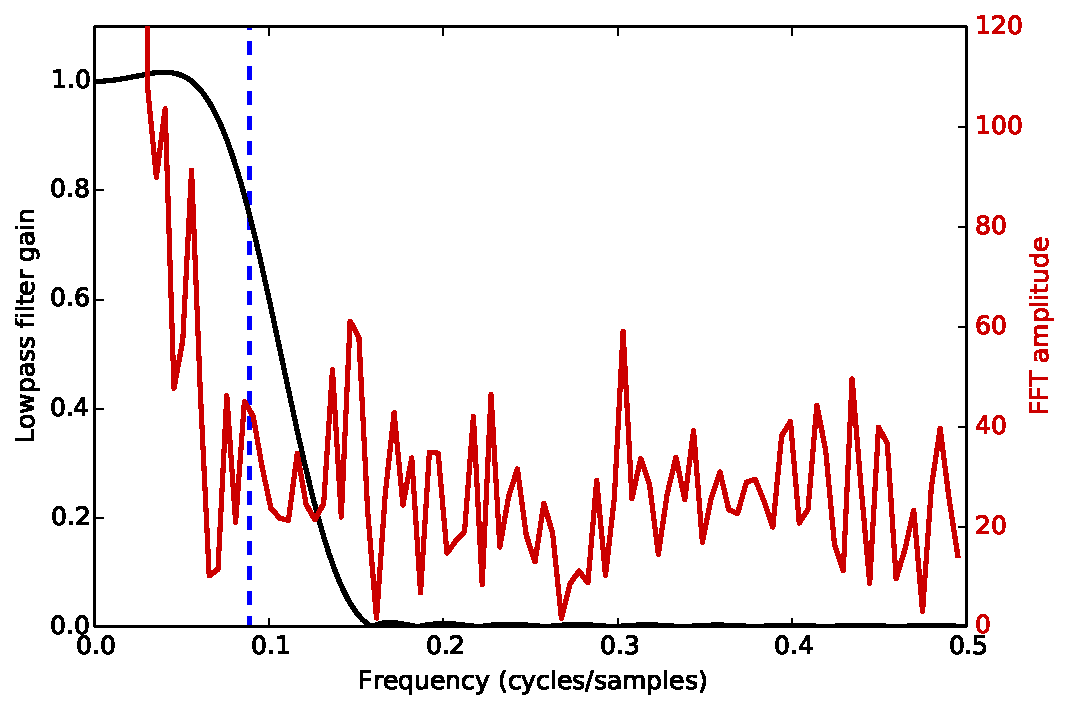
\includegraphics[scale=0.48]{fig/FIR_freq_resp_nmagse2_6.pdf}
	\caption{\label{fig_FIR}FIR filter designed for a track of length $N = 198$ samples.  The cutoff frequency of the track is shown as a blue vertical line.}
\end{figure}

As the magnitude of $B$ increases, the frequency of helical motion often becomes great enough that placing the filter
cutoff frequency $k_{c}$ near the cyclotron frequency does not permit sufficient filtering of the high-frequency
components of the track, and the resulting track is not smooth enough for a clean calculation of the curvature.
Thus we will often perform the analysis discussed in section \ref{ssec:curvature} using a lowpass filter with 
cutoff frequency of a fixed value for all magnetic field strengths, knowing that for the higher fields the resulting 
smoother track may be obtained at the expense of some information on the curvature induced by the field.

\subsection{Determination of the Track Curvature}\label{ssec:curvature}
The curvature at each hit in the track is calculated numerically by first separating the x-values, y-values, and z-values into their own arrays.  A lowpass FIR filter is designed to sufficiently smooth the track and applied to each of the arrays.  The derivatives $dx/dz$, $dy/dz$, $d^2x/dz^2$, and $d^2y/dz^2$ are calculated using the values in the array.  From these the curvature $\kappa$ is calculated at each point.  Since we do not have $x$ and $y$ as a function of $z$ but rather $x$, $y$, and $z$ as a function of hit number $n$, we can calculate the derivatives $x' \equiv dx/dn$, $y' \equiv dy/dn$, $z' \equiv dz/dn$ using the chain rule as $\frac{dx}{dz} = x'/z'$, and

\begin{equation}
\frac{d^2x}{dz^2} = \frac{x'' - z''(dx/dz)}{(z')^2}.
\end{equation}

The expressions for $dy/dz$ and $d^2y/dz^2$ can be obtained by replacing in the above $x \rightarrow y$.  Note that outliers may need to be removed from the resulting arrays of first and second derivatives due to points between which the z-coordinate changes very little.  To ensure more stable values of the derivatives, an outlier removal procedure is applied to all derivatives and second derivatives computed which consists of iteratively calculating the mean and variance $\sigma$ of each array, replacing any value that lies outside of $5\sigma$ of the mean value with the average of the two nearest values in the array, and continuing this procedure until the calculated variance $\sigma'^2$ is no longer less than the previous value of the variance $\sigma^2$. % (continue until $\sigma' < 0.99\sigma$).

The curvature calculated using each pair of points is then corrected as follows: if for the two points $z_2 < z_1$, that is $dz < 0$, the curvature is multiplied by -1 (see section \ref{ssec:magmotion}).  Note that the outlier removal procedure described above is also applied to the calculated curvature array.  Figure \ref{fig_trkcurv} shows the calculated curvature signs for a single-electron and double-beta event, after filtering with a lowpass filter.

\begin{figure}[!htb]
	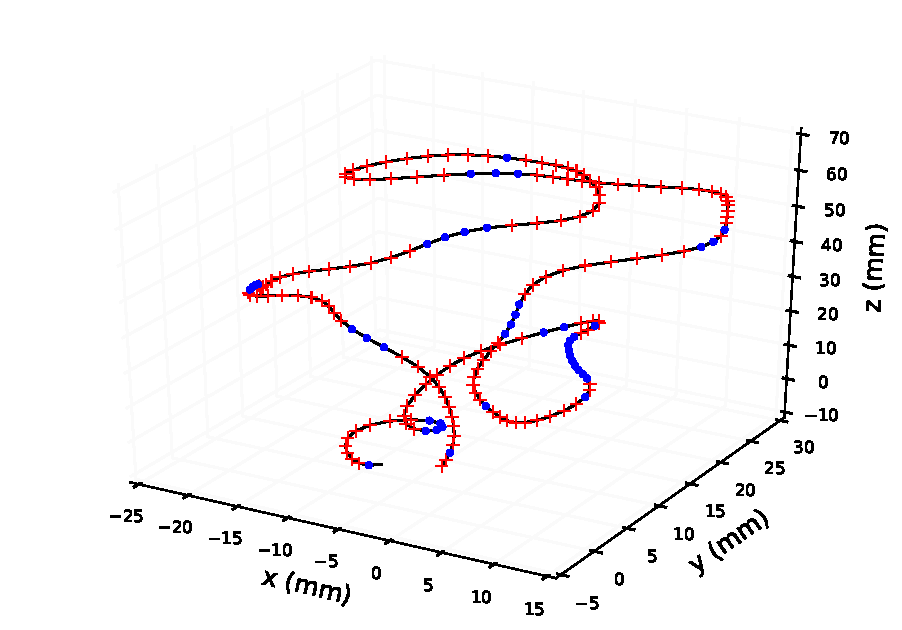
\includegraphics[scale=0.48]{fig/plt_trkcurv_nmagse2_6.pdf}
	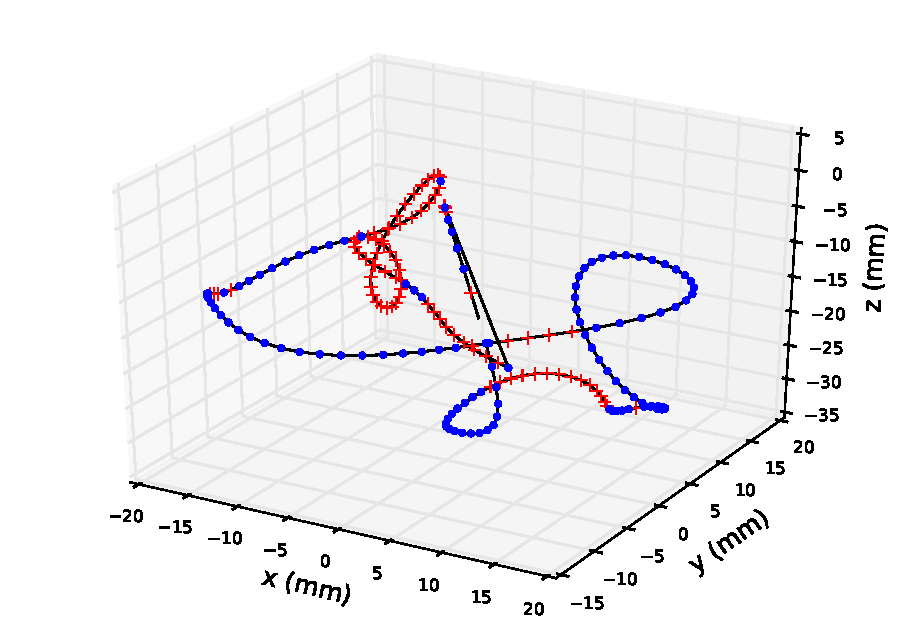
\includegraphics[scale=0.48]{fig/plt_trkcurv_nmagbb2_2.pdf}
	\caption{\label{fig_trkcurv}Calculated curvature sign at each point along the track for a single-electron event (left) and a double-beta event (right).  The red $+$ markers indicate positive curvature, while the blue dots indicate negative curvature.  Note that a lowpass filter has been applied to the tracks shown as described in section \protect\ref{ssec:FIR}.}
\end{figure}

A curvature sign array is created consisting of values of either $+1$ or $-1$ depending on the sign of each value in the calculated curvature array.  The curvature asymmetry factor is defined as the average of the curvature sign array using elements in the first half of the track minus the average of the curvature sign array using elements in the second half of the track.

\begin{equation}\label{eqn_assym}
\phi_{C} = \frac{1}{N/2}\Biggl(\sum_{i=0}^{N/2-1}\mathrm{sgn}(\kappa_{i}) - \sum_{i=N/2}^{N}\mathrm{sgn}(\kappa_{i})\Biggr).
\end{equation}

\noindent Note that if the number of hits in the track is odd, the first term includes the first $(N-1)/2$ hits and
the second term includes the remaining $(N-1)/2 + 1$ hits.

\section{Results: Background Rejection}
The analysis described in section \ref{sec:implementation} was performed for single-electron and
$0\nu\beta\beta$ tracks for all combinations of $P =$ 5, 10, and 15 atm and $B =$ 0.1, 0.3, 0.5, 0.7, 
and 1.0 T.  In all of these configurations, the hits were smeared in $(x,y)$ with $\sigma_{s} = 2$ mm and 
sparsed with $N_{s} = 2$.  Additional analyses in the $P =$ 10 atm, $B = 0.5$ T configuration were performed, 
one with $\sigma_{s} = 1$ mm and $N_{s} = 1$, and another with $\sigma_{s} = 3$ mm and $N_{s} = 3$.  For 
each configuration, 10000 events of each track type (single-electron and $0\nu\beta\beta$) were generated, 
and approximately 40-65\% of the tracks passed the initial topological cuts described in section 
\ref{ssec:track}.  The asymmetry factor shown in equation \ref{eqn_assym} was calculated for these tracks, and
a cut was placed on the calculated asymmetry factors defining the events considered to be candidate 
$0\nu\beta\beta$ tracks.  The cut was varied, and in each case 
the fraction of single-electron (background) tracks rejected by the cut was determined along with the fraction of 
$0\nu\beta\beta$ (signal) tracks accepted.\footnote{This is the fraction of the events that passed the initial 
topological analysis.  That is, we are considering the additional background rejection provided by this analysis  
once events of the chosen energy with a single continuous track have been selected out.}  An example of such 
an analysis is summarized in figure \ref{fig_svsbg}.

\begin{figure}[!htb]
	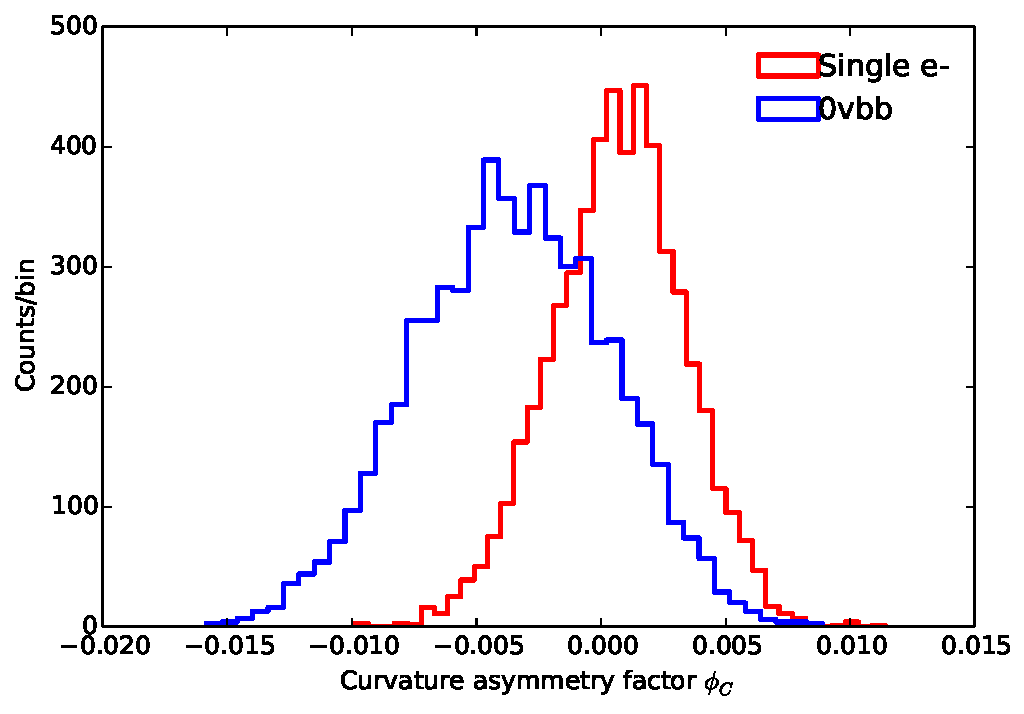
\includegraphics[scale=0.44]{fig/10atm_05T_scurv_diff_means.pdf}
	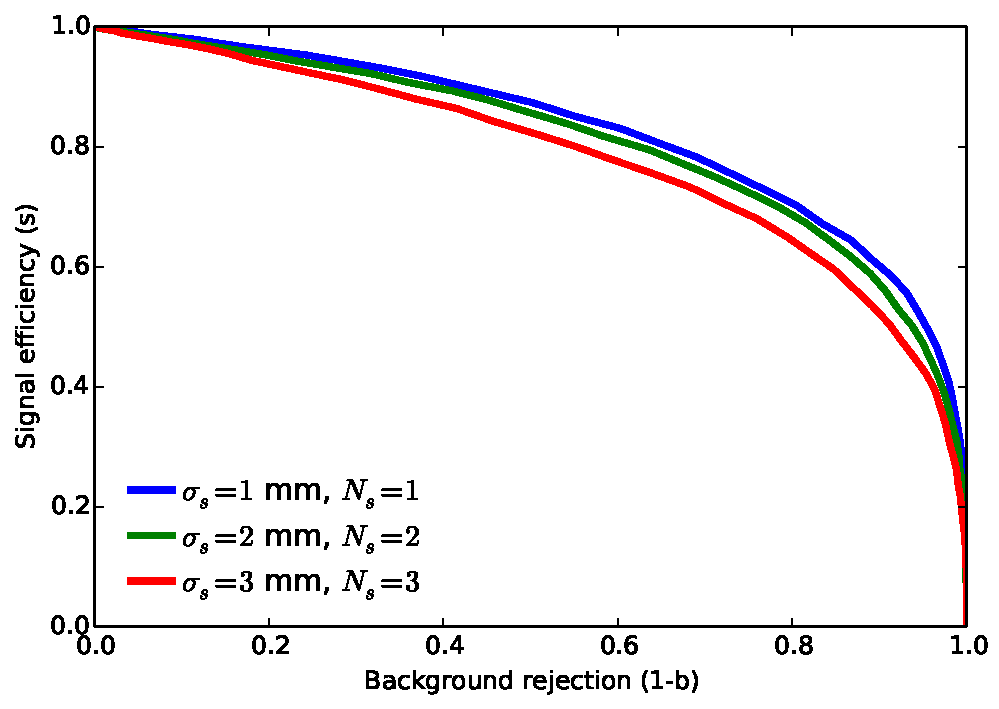
\includegraphics[scale=0.44]{fig/10atm_05T_sigvsb_all.pdf}
	\caption{\label{fig_svsbg}Curvature asymmetry factor for single-electron and $0\nu\beta\beta$ events with $\sigma_{s} = 2$ mm and $N_{s} = 2$ (left) and resulting signal efficiency vs. background rejection curve produced by varying a cut on $\phi_{C}$ space, shown also for $\sigma_{s} = 1$ mm and $N_{s} = 1$ and $\sigma_{s} = 3$ mm and $N_{s} = 3$ (right).  Here $s$ is the fraction of the total number of $0\nu\beta\beta$ events considered that was identified as a $0\nu\beta\beta$ event, and $b$ is the fraction of the total number of single-electron background events considered that was identifield as a $0\nu\beta\beta$ event.  These results were obtained for the $P = 10$ atm and $B = 0.5$ T configuration.}
\end{figure}

To demonstrate the performance of the method at the different configurations of gas pressure and magnetic 
field, we examine the signal efficiency $s$ (fraction of $0\nu\beta\beta$ events correctly identified) obtained 
given a cut that provides approximately 80\% and 90\% background rejection.  The results are shown in figure 
\ref{fig_config}.

\begin{figure}[!htb]
	\centering
	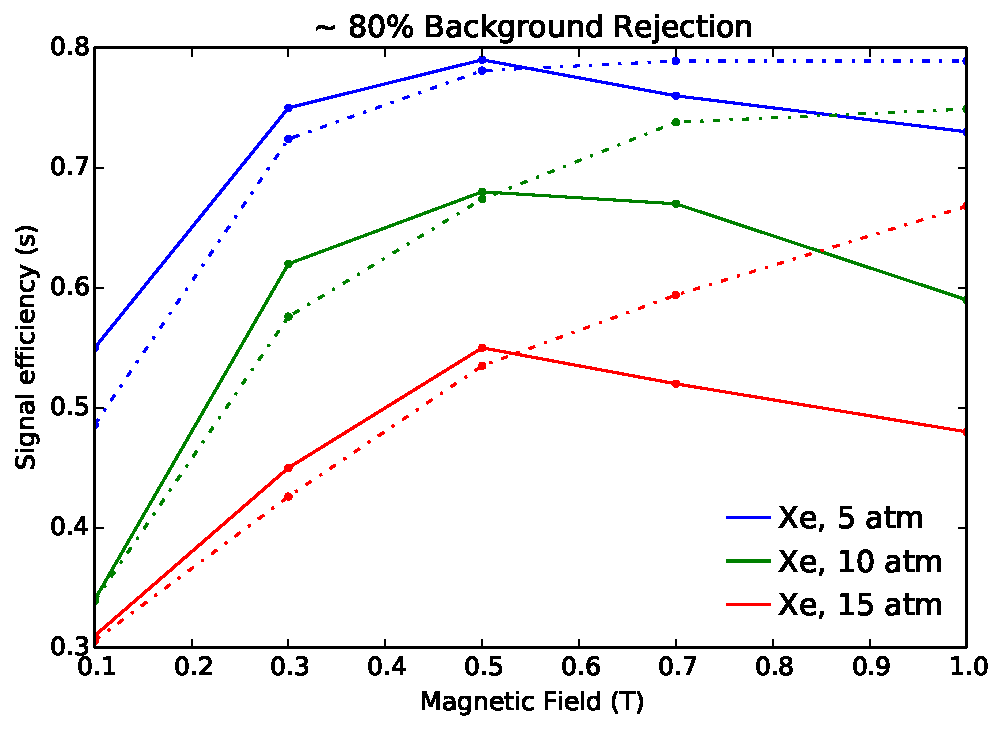
\includegraphics[scale=0.43]{fig/eff_vs_b_80.pdf}
	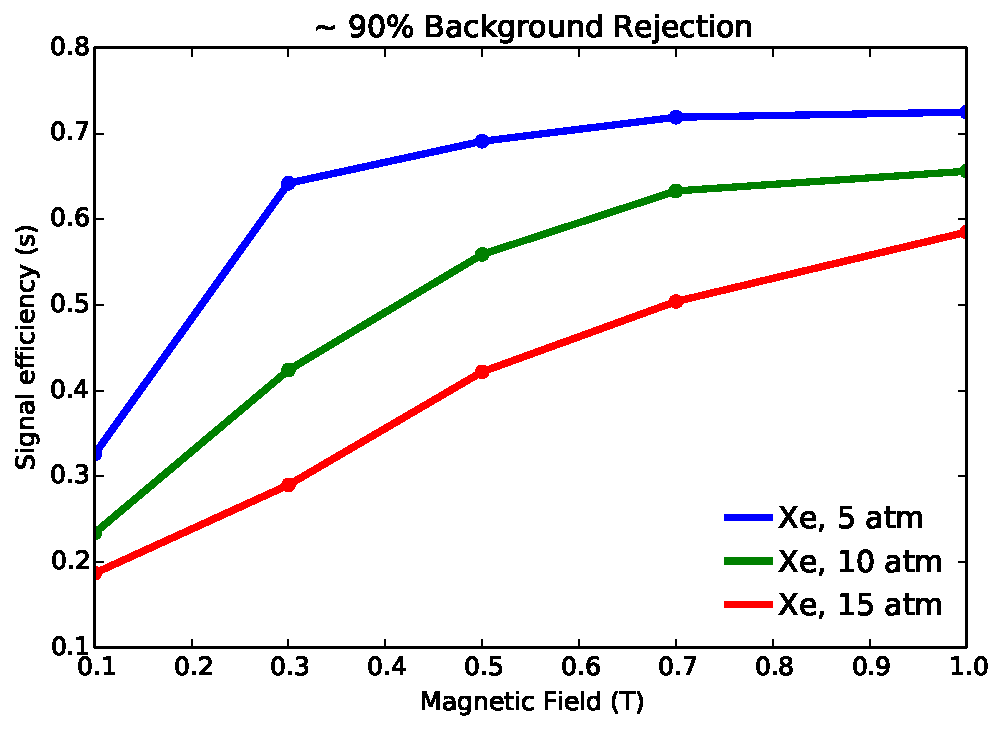
\includegraphics[scale=0.43]{fig/eff_vs_b_90.pdf}
	\caption{\label{fig_config}Signal efficiency corresponding to approximately 80\% background rejection (left) and 90\% background rejection (right) vs. magnitude of applied external magnetic field for different pressures.  The solid lines show the results of an analysis in which the lowpass filter applied varied from track to track, calculated using equation \protect\ref{eqn_kcyc}.  The dot-dashed lines show the results of an analysis in which $k_{\mathrm{cyc}}$ was fixed to a value of 0.085, a value representative of these simulated tracks for $B = 0.5$ T.}  % and $N_{s} = 2$.}
\end{figure}

\section{Conclusions}
The application of an external magnetic field in a high-pressure xenon detector capable of particle track reconstruction with resolution of approximately 2 mm in $(x,y,z)$ could present an additional background rejection factor of 80\% with an acceptable loss of signal efficiency at pressures of about 10 atm or less.  The background rejection improves with decreasing pressure due to the more extended tracks produced at lower gas densities.  For the lower pressures (5 atm and 10 atm), relatively little increase in signal efficiency is gained for an increase in magnetic field for fields greater than approximately 0.5 T.

Even an 80\% reduction in background would reduce the expected background rate in the NEXT experiment to
$1 \times 10^{-4}$ counts/keV/kg/year, or about 1 count/year for a 100 kg detector.  This warrants further
investigation, including the development of a discriminating variable more sophisticated than the asymmetry 
factor used in this study and application of this methodology to Monte Carlo data generated taking into account 
more aspects of the detector track reconstruction process.

\acknowledgments

This work was supported by the European Research Council under the Advanced Grant 339787-NEXT and the Ministerio de Econom\'{i}a y Competitividad of Spain under Grants CONSOLIDER-Ingenio 2010 CSD2008-0037 (CUP), FPA2009-13697-C04-04, FPA2009-13697-C04-01, FIS2012-37947-C04-01, FIS2012-37947-C04-02, FIS2012-37947-C04-03, and FIS2012-37947-C04-04.

\bibliography{nextb}

% Still to consider:
% - how does lower b.g. translate to sensitivity?


\end{document}